%-----------------------------------------------------------------------------%
\chapter*{Kata Pengantar}
%-----------------------------------------------------------------------------%
Dengan mengucap syukur kehadirat Allah SWT, saya dapat menyelesaikan skripsi ini sebagai salah satu syarat untuk menyelesaikan program studi Teknik Komputer di Universitas Indonesia. Penulisan skripsi ini tidak lepas dari dukungan dan bantuan berbagai pihak, yang dengan tulus saya ucapkan terima kasih.

Ucapan terima kasih yang sebesar-besarnya saya persembahkan kepada kedua orang tua saya, yang telah memberikan doa, dukungan moral, dan finansial selama proses pembuatan skripsi ini. Tak lupa kepada dosen pembimbing, Bapak Yan Maraden, S.T., M.T. atas bimbingan, arahan, dan kritik yang membangun selama proses penulisan skripsi ini.

Saya juga ingin mengucapkan terima kasih kepada teman-teman di Teknik Komputer Universitas Indonesia yang telah memberikan semangat dan dukungan. Pengalaman dan ilmu yang saya peroleh selama proses pembelajaran di universitas ini sangat berharga dan menjadi motivasi dalam penyelesaian skripsi ini.

Skripsi ini berjudul \judul yang merupakan upaya saya untuk memberikan kontribusi dalam bidang cloud serta sebagai aplikasi dari teori yang telah saya pelajari. Saya berharap skripsi ini dapat bermanfaat bagi pengembangan ilmu pengetahuan, khususnya bagi para peneliti dan mahasiswa yang berkecimpung dalam bidang yang sama.

Akhir kata, semoga skripsi ini dapat memberikan manfaat dan inspirasi bagi kita semua. Kritik dan saran yang membangun selalu saya harapkan untuk perbaikan di masa yang akan datang.


\vspace*{0.1cm}
\begin{flushright}
	Depok, 29 Desember 2023\\[0.1cm]
	\vspace*{1cm}
	\penulis
	
\end{flushright}
	
\iffalse
Template ini disediakan untuk orang-orang yang berencana menggunakan 
\latex~untuk membuat dokumen tugas akhirnya. 
Mengapa \latex? 
Ada banyak hal mengapa menggunakan \latex, diantaranya:

\begin{enumerate}
	\item \latex~membuat kita jadi lebih fokus terhadap isi dokumen, bukan 
		tampilan atau halaman. 
	\item \latex~memudahkan dalam penulisan persamaan matematis. 
	\item Adanya automatis dalam penomoran caption, bab, subbab, subsubbab, 
		referensi, dan rumus. 
	\item Adanya automatisasi dalam pembuatan daftar isi, daftar gambar, dan
		daftar tabel. 
	\item Adanya kemudahan dalam memberikan referensi dalam tulisan dengan 
		menggunakan label. Cara ini dapat meminimalkan kesalahan pemberian 
		referensi. 
\end{enumerate}

Template ini bebas digunakan dan 
didistribusikan sesuai dengan aturan \license, yang secara sederhana berisi: 

\begin{figure}
	\centering
	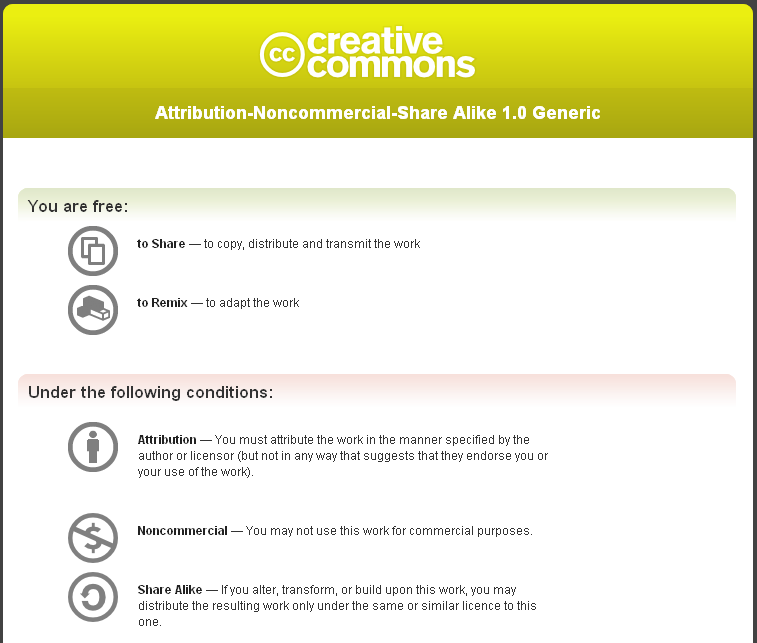
\includegraphics[width=0.74\textwidth]
		{assets/pics/creative_common.png}
	\caption{\license}
	\label{fig:lisensi}
\end{figure}

\pic~\ref{fig:lisensi} diambil dari 
\url{http://creativecommons.org/licenses/by-nc-sa/1.0/deed.en_CA}. 
Jika ingin mengentahui lebih lengkap mengenai \license, silahkan buka 
\url{http://creativecommons.org/licenses/by-nc-sa/1.0/legalcode}. 
Seluruh dokumen yang dibuat dengan menggunakan template ini sepenuhnya 
menjadi hak milik pembuat dokumen dan bebas didistribusikan sesuai dengan 
keperluan masing-masing. 
Lisensi hanya berlaku jika ada orang yang membuat template baru dengan 
menggunakan template ini sebagai dasarnya. 

Dokumen ini dibuat dengan \latex~juga. Untuk meyakinkan Anda, coba lihat 
properti dari dokumen ini dan Anda akan menemukan bagian seperti 
\pic~\ref{fig:pdflatex}. 
Dokumen ini dimaksudkan untuk memberikan gambaran kepada Anda seperti apa 
mudahnya menggunakan \latex~dan juga memperlihatkan betapa bagus dokumen 
yang dihasilkan. 
Seluruh url yang Anda temukan dapat Anda klik. 
Seluruh referensi yang ada juga dapat diklik. 
Untuk mengerti template yang disediakan, Anda tetap harus membuka kode 
\latex~dan bermain-main dengannya. 
Penjelasan dalam PDF ini masih bersifat gambaran dan tidak begitu 
mendetail, dapat dianggap sebagai pengantar singkat. 
Jika Anda merasa kesulitan dengan template ini, mungkin ada baiknya 
Anda belajar sedikit dasar-dasar \latex. 

\begin{figure}
	\centering
	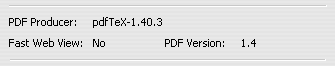
\includegraphics[width=0.54\textwidth]
		{assets/pics/mark.png}
	\caption{Dokumen Dibuat dengan PDFLatex}
	\label{fig:pdflatex}
\end{figure}

Semoga template ini dapat membantu orang-orang yang ingin mencoba menggunakan 
\latex. Semoga template ini juga tidak berhenti disini dengan ada kontribusi 
dari para penggunanya. 
Kami juga ingin berterima kasih kepada Andreas Febrian, Lia Sadita, Fahrurrozi 
Rahman, Andre Tampubolon, dan Erik Dominikus atas kontribusinya dalam template 
ini. 

\vspace*{0.1cm}
\begin{flushright}
Depok, 27 Februari 2019\\[0.1cm]
\vspace*{1cm}
\penulis

\end{flushright}
\fi